\subsection{RNA Synthesis}\label{sec:RNA_synthesis}
We now turn our attention to the next stage of the central dogma -- the
transcription of DNA to form RNA. We consider three major groupings
of RNA, namely the RNA associated with ribosomes (rRNA), the RNA encoding the
amino-acid sequence of proteins (mRNA), and the RNA which links codon
sequence to amino-acid identity during translation (tRNA).


rRNA serves as the catalytic and structural component of the ribosome,
comprising approximately 2/3 of the total ribosomal mass, and is decorated
with $\approx$ 50 ribosomal proteins. Each ribosome contains three rRNA
molecules of lengths 120, 1542, and 2904 nucleotides (BNID: 108093), meaning
each ribosome contains $\approx$ 4500 nucleotides overall. \textit{In vivo}
measurements of the kinetics of rRNA transcription have revealed that RNA
polymerases are loaded onto the promoter of an rRNA gene at a rate of
$\approx$ 1 per second (BNID: 111997, 102362). If RNA polymerases are
constantly loaded at this rate, then we can assume that $\approx$ 1
functional rRNA unit is synthesized per second per rRNA operon. While
\textit{E. coli} possesses 7 of these operons per chromosome, the fact that
chromosome replication can be parallelized means that the average dosage of
rRNA genes can be substantially higher (up to $\approx$ 70 copies) at fast
growth rates \citep{dennis2004}. At a growth rate of $\approx$ 0.5 hr$^{-1}$, however, the
average cell has $\approx$ 1 copy of its chromosome and therefore
approximately $\approx$ 7 copies of the rRNA operons, producing
$\approx$ 7 rRNA units per second. With a 5000 second division time, this
means the cell is able to generate around 3 $\times$ 10$^4$ functional rRNA
units, comparable within an order of magnitude to the number of ribosomes per
cell.

How many RNA polymerases are then needed to constantly transcribe the
required rRNA? If one polymerase is loaded per second, and the transcription
rate is $\approx$ 40 nucleotides per second (BNID: 101094), then the the
typical spacing between polymerases will be $\approx$ 40 nucleotides.
However, we must note that the polymerase itself has a footprint of $\approx$
40 nucleotides (BNID: 107873), meaning that one could expect to find one RNA
polymerase per 80 nucleotide stretch of an rRNA gene. With a total length of
$\approx$ 4500 nucleotides per operon and 7 operons per cell, the number of
RNA polymerases transcribing rRNA at any given time is then $\approx$ 500 per
cell.

As outlined in \FIG{RNA_synthesis}, and discussed further the Appendix
Section "\nameref{sec:SI_central_dogma}", synthesis of mRNA and tRNA together require
on the order of $\approx$ 400 RNAP. Thus, in total, one would expect the
typical cell to require $\approx$ 1000 RNAP to satisfy its transcriptional
demands. As is revealed in \FIG{RNA_synthesis}(B), this estimate is about an
order of magnitude below the observed number of RNA polymerase complexes per
cell ($\approx$ 5000 - 7000). The difference between the estimated number of
RNA polymerase needed for transcription and these observations, however, are
consistent with literature revealing that $\approx$ 80 \% of RNA
polymerases in \textit{E. coli} are not transcriptionally active
\citep{klumpp2008, patrick2015}, with the majority non-specifically bound to
DNA.

Our estimates also neglect other mechanistic features of transcription and
transcriptional initiation more broadly. For example, we acknowledge that
some fraction of the RNAP pool is nonspecifically bound to DNA during its
search for promoters from which to begin transcription. Furthermore, we
ignore the obstacles that RNA polymerase and DNA polymerase present to each
other as they move along the DNA \citep{finkelstein2013}. Additionally, while
they represent the core machinery for transcription, RNA polymerase is not
sufficient to initiate transcription. Initiation of transcription is
dependent on the presence of $\sigma$-factors, protein cofactors that bind
directly to the polymerase \citep{browning2016} and aid in promoter
recognition. In \FIGSUPP[RNA_synthesis]{sigma_70}, we show that the predicted
RNA polymerase copy number indeed is more comparable with the abundance of
$\sigma$-70 (RpoD), the primary sigma factor in \textit{E. coli}. There
therefore remains more to be investigated as to what sets the observed
abundance of RNA polymerase in these proteomic data sets. However, we
conclude that the observed RNA polymerase abundances are generally in excess
of what appears to be needed for growth, suggesting that the synthesis of RNA
polymerase themselves are not particularly limiting.

\begin{figure}
    \centering{
        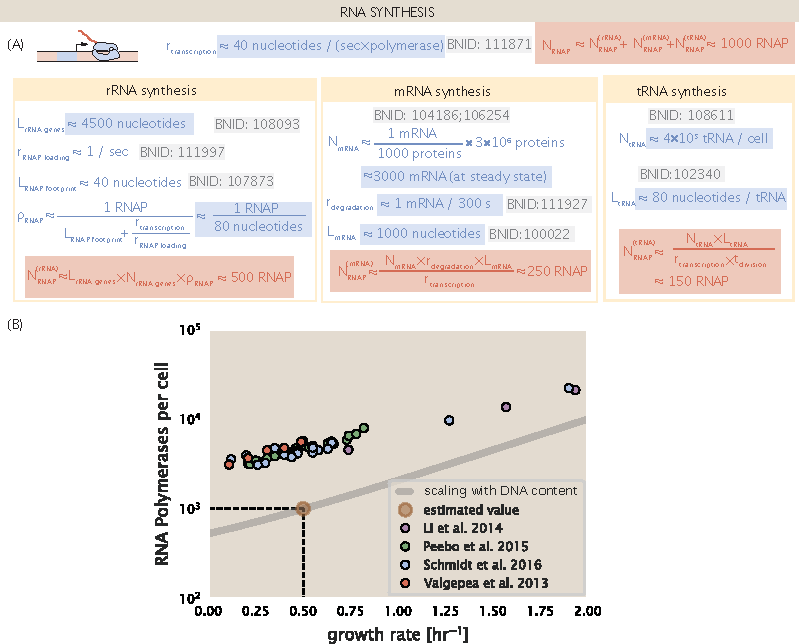
\includegraphics{main_figs/fig7_RNA_synthesis_main.pdf}
    }
        \caption{\textbf{Estimation of the RNA polymerase demand and
        comparison with experimental data.} (A) Estimations for the number of
        RNA polymerase needed to synthesize sufficient quantities of rRNA, mRNA,
        and tRNA from left to right, respectively. (B) The RNA
        polymerase core enzyme copy number as a function of growth rate. Colored
        points correspond to the average number RNA polymerase core enzymes that
        could be formed given a subunit stoichiometry of
        [RpoA]$_2$[RpoC][RpoB].} \label{fig:RNA_synthesis}

        \figsupp[Abundance and growth rate dependence of $\sigma$-70.]{The abundance of $\sigma^{70}$ as a function of growth rate.
        Estimated value for the number of RNAP is shown as a translucent brown
        point and grey line.}{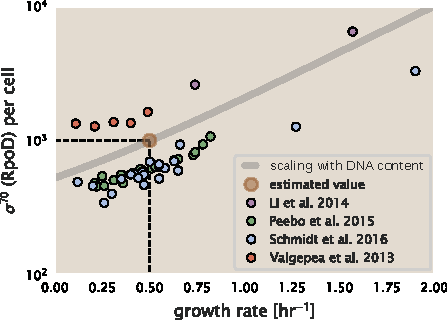
\includegraphics{main_figs/fig7-S1_sigma_factor.pdf}}\label{figsupp:sigma_70}

\end{figure}
